
%(BEGIN_QUESTION)
% Copyright 2014, Tony R. Kuphaldt, released under the Creative Commons Attribution License (v 1.0)
% This means you may do almost anything with this work of mine, so long as you give me proper credit

A student is asked to calculate the phase shift for the following circuit's output voltage, relative to the phase of the source voltage:

$$\includegraphics[width=15.5cm]{i01061x01.eps}$$

He recognizes this as a series circuit, and therefore realizes that a right triangle would be appropriate for representing component impedances and component voltage drops (because both impedance and voltage are quantities that add in series, and the triangle represents phasor addition):

$$\includegraphics[width=15.5cm]{i01061x02.eps}$$

The problem now is, which angle does the student solve for in order to find the phase shift of $V_{out}$?  The triangle contains two angles besides the 90$^{o}$ angle, $\theta$ and $\Phi$.  Which one represents the output phase shift, and more importantly, {\it why}?

\underbar{file i01061}
%(END_QUESTION)





%(BEGIN_ANSWER)

The proper angle in this circuit is $\theta$, and it will be a positive (leading) quantity.

\vskip 10pt

The reason we must focus on $\theta$ in this problem is because this is the angle separating the resistor's voltage drop from the source's voltage.  Note how in the circuit $V_{out}$ is measured across the resistor, not across the capacitor.

%(END_ANSWER)





%(BEGIN_NOTES)

Too many students blindly use impedance and voltage triangles without really understand what they are and why they work.  These same students will have no idea how to approach a problem like this.  Work with them to help them understand!

%INDEX% Electronics review: AC reactance and impedance

%(END_NOTES)


